\documentclass{suribt}
\title{ゲーム「2048」のプレイヤについて}
\author{金澤望生}
\eauthor{Kanazawa Nozomu}
\studentid{08-152021}
\supervisor{山口和紀 教授}
\handin{2018}{1}
\keywords{ゲームAI,機械学習}
\usepackage[dvipdfmx]{graphicx}
\usepackage{float}
\usepackage{algorithm}
\usepackage{algorithmic}
\usepackage{amsmath}

\begin{document}
\maketitle

\frontmatter
\begin{abstract}
インターネットブラウザやスマートフォン上で遊ぶことのできるパズルゲーム「2048」をプレイするAIの改良を行った.改良には盤面上で最も大きな数のタイルが隅にあることを重視する独自のヒューリスティック「corner bonus」を使用した.(仮)
\end{abstract}

\tableofcontents

\mainmatter
\chapter{導入}
モチベーションや2048の基本ルール・指標について説明します.

\section{モチベーション}
「2048」は,インターネットブラウザおよびスマートフォンなどの端末でプレイすることができるパズルゲームである.非常にシンプルで誰もが直感的にルールを理解できるのに対し,ゲームを理解したり安定して勝ち続けたりすることは非常に難しい2048は,その絶妙なバランスが評価されて非常に多くの人々が遊ぶようになった.同時に2048はゲームAI研究の対象としても活発に取り上げられるようになり,近年では強化学習を用いて訓練した非常に強いプレイヤが複数の研究者から発表されている.

これらのプレイヤの実装手法は汎用性が高く,他のゲーム(特に2048に類似したゲーム)や課題に対しても適用することが可能な手法が多く用いられている反面,人間が2048をプレイする際に用いている経験的な知識・方策は明示的に組み込まれていないことが多い.一部の先行研究においては特徴量として人間が注目する指標を組み込んでいるものの,これらの指標も強化学習によって訓練されるため,経験的な知識が学習によって獲得されると言うことはできない.

そこで,本研究においては,これまでに発表されてきた強化学習で訓練を行う2048プレイヤに対して,人間による経験的な知識をトップダウン型で組み込むことにより,計算機によってのみ訓練されたプレイヤよりも強いプレイヤを実装し,新たな側面から2048の自動プレイヤに改良の余地があることを示すことを目的とする.

\section{2048について}
2048がGabriele CirulliによってGitHub上に公開されたのは2014年3月のことである.Cirulliは2048を開発していた当時,「1024」および「2048」\footnote{Cirulli自身が発表した2048とは似ているが,ルールが異なる別のゲームである}というゲームに熱中していた.これらのゲームはどちらもAsher Vollmerによるゲーム「Threes」にルールがよく似ている類似作品であるが,Cirulliは当時Threesの存在については認識していなかった.CirulliはこれらのThreesに端を発するゲームを改良するべく新たなゲームを開発し,ついに「2048」として公開することとなった.ここで挙げた1024,Cirulliが参考にした2048,そしてCirulli自身が発表した2048は全てThreesの類似作品であるものの,これらの作品群の中ではCirulliによる2048が最も人気を集めており,全世界で2300万人以上の人が2048\footnote{なお,ここから単に2048と表記した場合,それはCirulliが開発した2048のことを指す}で遊んだとされる.

2048はシンプルで直感的にルールを理解できる一方で,マスターすることが非常に難しいゲームであることが特徴となっており,このために多くのプレイヤーを熱中させていると同時にゲームAI研究の題材としても多く取り上げられていると考えられる.また,ゲームとしての2048について着目すると,2048については以下のような特徴を挙げることができる:

\subsubsection{完全情報ゲームである}
2048は単一の状態から始まり,1人のプレイヤが自分の手番で何かしらの行動を起こすことによって状態が遷移し,さらにプレイヤはゲームの状態を全て把握することができる.したがって,2048は完全情報ゲームであると言える.

\subsubsection{非決定論的ゲームである}
2048は1人のプレイヤによってのみプレイされるゲームであるが,状態の変化の際には乱数によって決定される要素があるため,プレイヤは次の状態を知ることはできない.したがって,2048は非決定論的(nondeterminisitc)ゲームである.ただし,プレイヤは次の状態がいくつあり,その状態にどれぐらいの確率で遷移するのか自分で計算することはできる.

\subsubsection{明確な終局が予め設定されていない}
チェスや将棋といったゲームについては,どのような状態に到達するとゲームが終了するのか規定されており,プレイヤはお互いに相手を終局に向かわせることを念頭にゲームをプレイする.一方で,2048には次の状態に遷移することが不可能になったらゲームが終了するというルールはあるものの,その状態に到達するまでは無限にゲームを進めることができる.すなわち,プレイヤが熟達すればするほど長い時間ゲームを進めることができ,その分プレイヤの優秀さを示す指標も良くなる.この特徴により,2048は強化学習やゲームAIのベンチマークとしてよく機能していると考えられる.

\section{2048のルール}


\chapter{先行研究の紹介}
既存研究が使用している手法とプレイヤの成績について説明します.(編注・提出原稿では以下は削除)なお,JaskowskiはJa\'{s}kowskiが正しい表記ですが,差し当たりJaskowskiと表記し,最後にまとめて正しい表記に置換します.

\section{Szubert \& Jaskowski (2014)}
Szubert \& Jaskowskiは,TD学習を用いたプレイヤの訓練とnタプルネットワークを用いた価値関数の表現を組み合わせることによって,人間の知識やゲーム木探索を使用しないで十分強い2048プレイヤを実装することに成功した。
\subsection{TD学習}
TD学習の「TD」とはtemporal differenceの略であり,すなわち状態間における価値の差分を学習することによって学習器の訓練を行う手法である。2048にあてはめると,とある盤面$s'$の価値と,その盤面の1プレイ後の盤面$s'_{next}$の価値の差分を取り,これを現状定まっている$s'$に足し込んでいくことで訓練を行うことになる。TD学習にはさまざまな派生があるが,Szubert \& Jaskowskiが使用しているTD(0)学習は以下の式によって表現される:

\[
	V(s) ← V(s) + \alpha (r + V(s'') - V(s) )
\]

この式において,$V$は価値関数,$\alpha$は学習率,$r$は報酬である。学習率は計算された差分を価値関数の更新にどれほど反映するかを決定するパラメータである。

TD学習はTesauroによるバックギャモンへの適用でよく知られるようになり,碁やオセロ,チェスにおけるゲームAIの方策決定の手法として用いられるようになった。

\subsection{nタプルネットワーク}
TD学習によって盤面の評価とその学習を行うことができるが,盤面と評価値をどのように結びつけるかが問題になる。まず,2048で有り得るすべての盤面に対して評価値を与える1対1対応のルックアップテーブル(LUT)を作成することを考えると,2048で有り得る盤面の数は$(4 \times 4)^{18} \approx 4.7 \times 10^{21}$と膨大な数になり,このようなLUTを計算機上で実装することは現実的に不可能である。

そこで,一部のマスの組み合わせによる「タプル」というクラスターを作成し,さらに複数のタプルを組み合わせることで盤面を表現する手法「nタプルネットワーク」を2048に導入することが,Szubert \& Jaskowskiによって提案された。たとえば,図\ref{figure_001}のようなnタプルネットワークを実装した場合,1つのゲーム内で保持すべき重みの数は860625であり,全ての有り得る盤面に対するLUTを保持するのに対して非常に少なくて済む。

\begin{figure}[t]
	\begin{center}
	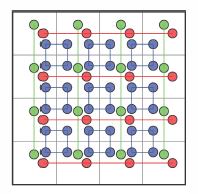
\includegraphics[width=5cm]{figure_001.png}
	\caption{nタプルネットワークの例}
	\label{figure_001}
	\end{center}
\end{figure}

nタプルネットワークはBledsoe \& Browning (1959)によりパターン認識に用いられたのが最初の採用例である。ゲームAIの分野ではJaskowski (2014)によってオセロに適用され,一定の成果が得られた。

\subsection{結果と課題}
本手法をもとに行った実験のうち,最も良い勝率を達成したプレイヤを用いて10万ゲーム中の成績を検証したところ,勝率は0.9781であり,平均スコアは100,178であった.1ゲーム中に達成されたスコアで最も良かったのは261,526であった.Szubert \& Jaskowskiによる新たな手法は探索ベースの手法よりも大幅に高速で,かつ成績が良かった.

しかしながら,この手法では「常に2048-tileを生成すること」よりも「時々16384-tileを生成すること」を重視しているため,勝率は必ずしも100\%を達成できていない.また,人間の知識を一切導入していないため,最も大きな数のタイルが盤面上の端に配置されないなど,人間の直感的な戦略とは反しているといったデメリットがあった.

\section{Wu et al. (2014)}
Wuは,Szubert \& Jaskowskiの手法を改良し,木探索を用いた先読みと組み合わせることによってさらに良いプレイヤを実装することに成功した.

\subsection{nタプルネットワークの配置の改善}
Wuは,Szubert \& Jaskowskiが考案したnタプルネットワークのうち,直線型で4タプルとして配置していたタプルを,図\ref{figure_002}(b)のように柄杓型の6タプルに変更した.これによって増える重みの数は約2倍程度であったが,この変更によってSzubert \& Jaskowskiのものよりも飛躍的に良い成績を得ることができた.なお,なぜこのようなタプルの配置が最善だと判断したのかについて,Wuは論文において言及していない.

\begin{figure}[t]
	\begin{center}
	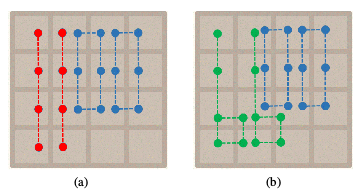
\includegraphics[width=8cm]{figure_002.png}
	\caption{Szubert \& Jaskowski(a)とWu(b)が提唱したnタプルネットワーク}
	\label{figure_002}
	\end{center}
\end{figure}

\subsection{Multi-Stage TD学習の導入}
Multi-Stage TD学習(MS-TD学習)とは,ゲームの局面に応じて異なる価値関数を保持することによって,よりそれぞれの局面に対して適切な重みを学習させることを目的とした手法である.Wuは学習のプロセスを3つのステージに分割し,ゲームプレイも同様に3つのステージに分割して行うようにした.Wuの提唱した2048におけるMS-TD学習は,以下のような手順で学習を行う.なお,「$T_{16k}$」とは「そのゲーム中で初めて16384-tileを生成することに成功した時」,「$T_{16+8k}$」とは「そのゲーム中で初めて16384-tileを生成した後に,初めて8192-tileを生成することに成功した時」のことを示す.

\begin{enumerate}
\item 第1ステージにおいては,初期盤面からゲームを始めて,価値関数が十分飽和するまで学習を行う.このステージで学習された価値関数の重みのことを「Stage-1価値関数」と呼ぶことにする.また,学習ゲーム中に$T_{16k}$を達成したなら,その時の盤面を全て保存しておく.
\item 第2ステージにおいては,第1ステージで保存した盤面からゲームを始めて,TD学習を行う.このステージで学習された価値関数の重みのことを「Stage-2価値関数」と呼ぶことにする.また,学習ゲーム中に$T_{16+8k}$を達成したなら,その時の盤面を全て保存しておく.
\item 第3ステージにおいては,第2ステージで保存した盤面からゲームを始めて,TD学習を行う.このステージで学習された価値関数の重みのことを「Stage-3価値関数
」と呼ぶことにする.
\end{enumerate}

その後,以下のような手順でゲームプレイを行う.

\begin{enumerate}
\item 盤面が$T_{16k}$を達成するまでは,Stage-1価値関数を用いてゲームプレイを行う.
\item 盤面が$T_{16k}$を達成してから$T_{16+8k}$を達成するまでは,Stage-2価値関数を用いてゲームプレイを行う.
\item 盤面が$T_{16+8k}$を達成してからは,Stage-3価値関数を用いてゲームプレイを行う.
\end{enumerate}

\subsection{Expectimax木探索}
Szubert \& Jaskowski (2014)によって,木探索ベースの2048プレイヤは強化学習で訓練したプレイヤに劣ることが示されたが,Wuは強化学習によるプレイヤに対してExpectimax木探索を補助的に組み合わせることによって,さらにプレイヤの性能を高めようと試みた.

\begin{figure}[t]
	\begin{center}
	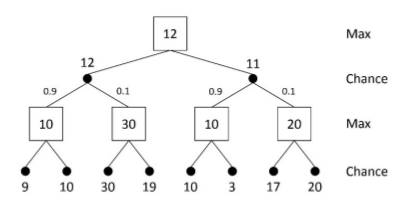
\includegraphics[width=8cm]{figure_003.png}
	\caption{Expectimax木の例 (Wu et al. (2015))}
	\label{figure_003}
	\end{center}
\end{figure}

Expectimax木探索には,MaxノードとChanceノードという2種類のノードがあり,それぞれのノードの値は子ノードから決定される.Maxノードの値は,子ノードのうち最も大きな値のノードの値となる.例えば図\ref{figure_003}の根ノードの値は12であるが,これは子ノードの「12」と「11」のうち最大の値である12を取ったものである.一方でChanceノードの値は子ノードの期待値となる.例えば図\ref{figure_003}の根ノードの子ノードの1つである「12」というノードは,0.9の確率で10となるノードと0.1の確率で3となるノードの期待値,すなわち$0.9 \times 10 + 0.1 \times 3 = 12$によって12という値が決定する.

Wuの提案においては,Maxノードの値はプレイヤがアクションを選択して遷移を行った後の盤面,Chanceノードは遷移を行った後にランダムタイルを発生させた後の盤面が与える評価値となる.例えば,ある盤面$s$(アクション選択と遷移が終わった直後の盤面とする)の評価値を深さ3のExpectimax木探索を用いて求めたい時,図hogehogeのような探索木が考えられる.$s$の盤面が分かれば,その子ノードであるランダムタイル生成後の盤面,さらにその子ノードである遷移後の盤面を求めることができる.さらに,葉ノードにあたるChanceノードの値は価値関数が与える評価値とすることで,各ノードの値を求めることができ,最終的に根ノード,すなわち評価値を求めたい盤面$s$の評価値も求められるということになる.

(図2.4. 何かいい感じの2048の探索木を自分で描画して貼る)

Expectimax木探索を用いて先読みをすることで,将来の盤面を予想してより良いアクションを選択できるようになった.これはスコアの面での成績が良くなることに繋がる一方で,maxTile=2048を達成する割合,すなわち勝率の向上にも大きな影響をもたらした.

\subsection{結果と課題}
WuによるプレイヤはSzubert \& Jaskowskiのものに比べて著しく良い成績を達成した.まずSzubert \& Jaskowskiが達成できなかった32768-tileの生成に成功し,10.9\%の確率で32768-tileを生成できるようになった.勝率に関しては1を達成,すなわち2048-tileは100\%の確率で生成できるようになり,平均スコアは328,946,最大スコアは605,752を記録した.これは当時としては1つの例外\footnote{Xiaoによる深深度先読みと人間による調整を行った評価関数を用いたプレイヤがこれにあたるが,Wuのものよりも100倍遅い:https://www.youtube.com/watch?v=JQut67u8LIg}を除き,計算機による2048プレイヤの中で最も優れた成績であった.

一方で,nタプルネットワークの形状変更やMS-TD学習のステージングについては,この研究で行なわれた調整についてこれといった根拠が述べられておらず,依然として改良の余地は残していた.特にnタプルネットワークの形状変更については,次のOka \& Matsuzakiの研究で詳しく検討されることとなった.

\section{Oka \& Matsuzaki (2016)}
Szubert \& Jaskowskiは当初図\ref{figure_001}のようなnタプルネットワークを考案していたが,このnタプルネットワークによる学習器はあまり性能が高くなく,平均スコアは10万ゲーム学習した時点で5万〜6万程度にとどまっていた.そこで,図\ref{figure_002}(a)のようなnタプルネットワークへの改良が行われ,その結果平均スコア・勝率ともに改善することができた.さらにWuはSzubet \& Jaskowskiの考案したnタプルネットワークを改良し,成績を伸ばすことができた.

しかしながら,ここまでは「タプルのサイズを大きくすると学習器の成績も良くなる」という大まかな関係しかわかっておらず,成績を最善にするnタプルネットワークはどのような形状になるのか厳密には検討されていなかった.これを厳密に検討したのがOka \& Matsuzakiである.

\subsection{nタプル単体の性能の評価}
Oka \& Matsuzakiは,まずnタプル単体の性能を網羅的に評価することを目指した.2048の盤面上でn個のタイルを選んで形成されうるnタプルの数は,表\ref{tab:ntuplesNumber}の通りとなっている.

\begin{table}[t]
	\begin{center}
		\caption{形成されうるnタプルの数}
		\begin{tabular}{l|r|r|r|r|r|r|r|r|r|r|r} \hline
		N & 3 & 4 & 5 & 6 & 7 & 8 & 9 & 10 & 11 & 12 & 13 \\ \hline \hline
		All & 77 & 252 & 567 & 1051 & 1465 & 1674 & 1465 & 1051 & 567 & 252 & 77 \\ \hline
		Connected & 8 & 17 & 33 & 68 & 119 & 195 & 261 & 300 & 257 & 169 & 66 \\ \hline
		\end{tabular}
		\label{tab:ntuplesNumber}
	\end{center}
\end{table}

ここで,Connectedとはタプル上の全てのタイルが1個以上の他のタプルの接していることを指す.Oka \& MatsuzakiはConnectedタプルのうち,十分性能が良く,なおかつ現実的にnタプルネットワークとして運用することができる$N=6$と$N=7$の場合のみ検討することとした.彼らは次に,形成されうるConnectedな6タプル68個の中からランダムに10個のタプルを選んで100万ゲームの学習を行う実験を680回\footnote{$680 \times 10 = 6800$より,全てのタプルが100回は選ばれるようにするため}繰り返し,各タプルの性能を比較可能な数値として算出した.7タプルについても同様な実験を行った.

その結果,6タプルと7タプルのうち最も優れた4つのタプルと最も劣った4つのタプルが,図\ref{figure_004}の通り明らかになった.

\begin{figure}[t]
	\begin{center}
	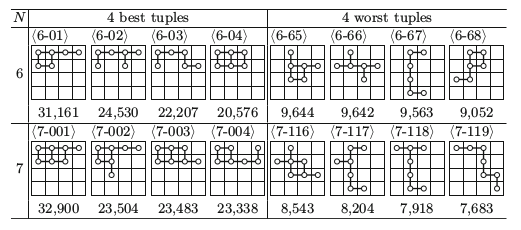
\includegraphics[width=10cm]{figure_004.png}
	\caption{最も優れている/劣っている上位4つの6タプル・7タプル (Oka \& Matsuzaki (2016))}
	\label{figure_004}
	\end{center}
\end{figure}

\subsection{nタプルネットワークに組み込むnタプルの数の検討}
6タプルおよび7タプルの性能が判明したので,性能が良い任意の数のタプルを組み合わせてnタプルネットワークを作成することが可能になった.Szubert \& JaskowskiおよびWuは4個のタプルを組み合わせてnタプルネットワークを作成していたが,Oka \& Matsuzakiは5個以上のタプルを組み合わせることを検討した.すなわち,nタプルの数が多くなればなるほどnタプルネットワーク全体としての性能も上がると思われるが,最も性能が良くなるタプルの数は何個かを明らかにするということである.

実験においては,6タプルの場合最大で上位45個,7タプルの場合最大で上位10個のタプルからnタプルネットワークを作成することとした.各nタプルネットワークに対して,600万ゲーム学習を行わせ,10,000ゲームごとに平均スコアと最大スコアを記録した.その結果が図\ref{figure_005}である.なお,mは実験を行うにあたって上位m個のnタプルを採用してnタプルネットワークを生成したことを示す.

\begin{figure}[t]
	\begin{center}
	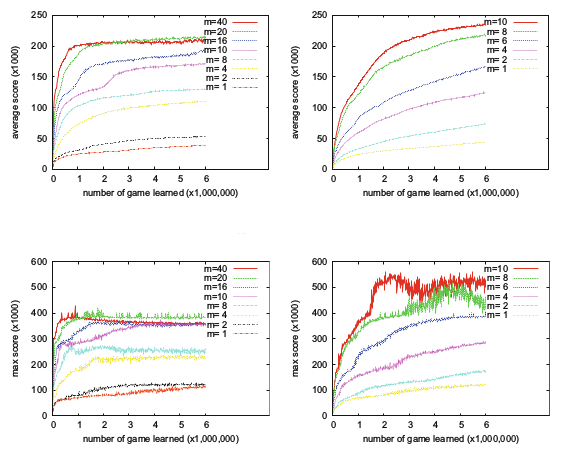
\includegraphics[width=10cm]{figure_005.png}
	\caption{成績上位タプルm個を組み合わせたタプルネットワークの実験 (Oka \& Matsuzaki (2016))}
	\label{figure_005}
	\end{center}
\end{figure}

上記の通り,実験群の中では10個の7タプルを組み合わせたタプルネットワークが最も良い成績を収めることがわかった.なお,グラフからも読み取れるが,7タプルによるネットワークに関しては600万ゲーム学習しても平均スコア・最高スコアが収束しない.そのためさらに組み合わせるタプルを増やすとさらに成績が良くなることが考えられるが,技術上の制約により$m=11$以上は実現できなかった\footnote{7タプルを組み合わせてタプルネットワークを作成する場合,重みを保持するために1個のタプルにつき1GBのメモリを消費しなければならない.Oka \& Matsuzakiが実験を行った環境はメモリが12GBしか確保できなかったため,$m=11$以上は実験を行うことが困難だったのではないかと考えられる.また,この研究においてゲーム木探索を組み込むことができなかったのもメモリの制約が原因ではないかと考えられる}.

\subsection{結果と課題}
Oka \& Matsuzakiの研究における最も良いnタプルネットワークは,勝率が0.9850,平均スコアが234,136,最高スコアが504,660という成績を残した.これはゲーム木探索を用いない計算機を用いた2048プレイヤとしては最も良い成績であった.しかしながら,ゲーム木探索を用いなかったことによりゲーム序盤では安定性を欠いてしまい,Wuが達成した勝率1を割り込む形となってしまったし,単純に2048プレイヤとしての成績を比べるとWuのものよりも平均スコア・最大スコアともに低くなっている.一方で,ゲーム木探索を採用しなかったことはプログラムの高速化という点では利があり,1秒あたり88000手の遷移を行うことができるプログラムとなった.これはWuの研究と比べて約290倍高速である.

\section{Yeh et al. (2016)}
YehはWu et al. (2014)の研究にも参画していた共同研究者で,Wuの研究の流れを引き継ぐような形で2048プレイヤの改良を行った.Wuの研究で用いたMS-TD学習の考え方,改良されたnタプルネットワーク,Expectimax木探索は引き続き用いられているため,この研究で新たに加わった要素のみを述べる.

\subsection{新たな特徴の追加}
Yehは,nタプルネットワークによる学習の他に,盤面に現れた特徴を評価関数として用いることとした.盤面の評価値には従来のnタプルネットワークによる評価値と新たに採用した特徴による評価関数の和を用い,これをTD学習で訓練した.なお,採用した特徴は以下のつである.

\begin{enumerate}
\item 大きな数が書かれたタイルの個数
\item 何も書かれていないタイルの個数
\item 異なる数が書かれた(distinct)タイルの個数
\item マージすることができるタイルのペアの組数
\item 書かれているタイルの数が$(n, 2n)$の形になっているタイルのペアの個数
\end{enumerate}

\subsection{MS-TD学習のステージングの改良}
WuはMS-TD学習を行うにあたり3ステージに分けて訓練・ゲームプレイを行っていたが,このステージの分け方をさらに細かくした.Yehによってテストされたステージングは以下の通りである.なお,$T_{x+y+zk}$という表記は,「盤面に初めて$1000x, 1000y, 1000z$のタイルが同時に現れた時」のことを指す.各タイルの数は百の位で切り捨てられて表現されている.

\begin{enumerate}
\item 4ステージ:$T_{8k}, T_{16k}, T_{16+8k}$を境界としてステージを分ける
\item 4ステージ:$T_{16k}, T_{16+8k}, T_{16+8+4k}$を境界としてステージを分ける
\item 5ステージ:$T_{16k}, T_{16+8k}, T_{16+8+4k}, T_{16+8+4+2k}$を境界としてステージを分ける
\item 6ステージ:$T_{16k}, T_{16+8k}, T_{16+8+4k}, T_{16+8+4+2k}, T_{16+8+4+2+1k}$を境界としてステージを分ける
\end{enumerate}

これらのステージングを,上から順に戦略1から戦略4とする.まず戦略1をテストした際,$T_{8k}$を境界としてステージを分けることは意味がないことがわかったため,戦略2以降では$T_{16k}$以降のステージングのみを考えることとした.戦略2から戦略4をテストした結果,平均スコアでは戦略4が最も優秀であることがわかったが,最高スコアと32678-tileの到達率では戦略3が最も優秀であった.各戦略ごとの成績は表hogehogeの通りである.

(表hogehogeをここに書きます)

以上の結果より,Yehは戦略3が最も優れたステージングだと判断し,これ以降は戦略3を用いて実験を行った.

\subsection{学習率の調整}
TD学習をより正確に行うために,まず学習率$\alpha = 0.0025$でTD学習を行った後,価値関数に大きな改善が見られなくなったと判断したら,学習率$\alpha = 0.00025$に変更して学習を続行させるようにした.

\subsection{$TD(\lambda)$の使用}
Szubert \& JaskowskiおよびWuはTD学習においてTD(0)を使用していたが,YehはTD(0.5)を用いて5ステップの報酬を平均化することとした.すなわち,

(ここに数式を書きます)

で表現される$R^{\lambda}_t$を用いてTD学習を行うようにした.

\subsection{結果と課題}
上記の改良を重ねた結果,Yehは平均スコア443,526,最大スコア793,835と非常に良い成績の学習器を訓練することに成功した.なお,32678-tileへの到達率は31.75\%,1秒あたりの遷移速度は500手であった.さらに,検証ゲーム中のある1ゲームにおいて65536-tileを生成することにも成功した.これは強化学習ベースの2048プレイヤでは当時として最も強く,Xiaoのよる深深度探索ベースのものよりも平均スコアでは優っており,Yehの方が125倍速いプログラムであった.

\section{Jaskowski (2017)}
Jaskowskiは,Yehまでの2048プレイヤの改良の流れを受け継ぎながら,これまで用いられてきたTD学習や訓練・検証のステージングなどに対して改良を加えつつ,新たな手法を加えることでさらに優秀なプレイヤの実装を目指した.

\subsection{自動的な学習率決定アルゴリズムの適用}
JaskowskiはTD(${\lambda}$)を使用する点はYehの研究を継承したが,TD学習で最も重要なパラメタである学習率を決定するにあたり,新たな手法を提案した.すなわち,Yehの研究では手動で学習率が設定されていたのに対して,Jaskowskiはこれまでに提案されてきたオンライン適応学習による学習率決定のアルゴリズムを2048にも適用することを試みた.

Bagheri et al.によるConnect 4への適用の研究において,これらの学習率決定アルゴリズムはいずれも標準的なTD学習よりも良い成績を残すことが明らかとなったが,一方で長期的に見るとアルゴリズム間の差はそこまで大きいものにはならなかった.そこで,Jaskowskiは最もシンプルなTemporal Coherence(TC(${\lambda}$))と,より先進的でチューニングの必要がないAutostepを選択して実験することにした.

\subsubsection{TC(${\lambda}$)}
これまでのTD(${\lambda}$)では実験者が学習率${\alpha}$を手動で決定していたが,TC(${\lambda}$)においては,手動で決定される${\alpha}$の代わりに以下のパラメータを用いて学習率${\gamma}$を決定する.

\begin{itemize}
\item \textbf{メタ学習率${\beta}$}:実験者が手動で設定するパラメータ
\item \textbf{累積誤差関数$E(s)$}:これまでTD学習で価値関数$V(s)$の更新を行う際に用いてきた誤差${\delta}_t = r_{t+1} + V(s_{t+1}) - V(s_t)$を,$V(s)$の更新を行う際に$E(s)$に対して加算する.盤面$s$は価値関数と同様に,nタプルネットワークを用いて近似される
\item \textbf{累積絶対誤差関数$A(s)$}:$V(s)$の更新を行う際に,${\delta}_t$の絶対値を$A(s)$に対して加算する.盤面$s$は価値関数と同様に,nタプルネットワークを用いて近似される
\item \textbf{適応学習率${\alpha}$}:$E(s)$と$A(s)$の値によって自動的に決定されるパラメータ
\end{itemize}

適応学習率${\alpha}$は以下の式で求められる.

\[
{\alpha} = 
\begin{cases}
\dfrac{|E_i[s'_k]|}{A_i[s'k]}, & \text{if $A_i[s'k] \neq 0$} \\
1 & \text{otherwise}
\end{cases}
\]

また,学習率${\gamma}$は以下の式で求められる.

\[
{\gamma} = \dfrac{{\alpha} \times {\beta}}{m} \text{($m$はnタプルネットワークに格納されているタプルの数)}
\]

このような学習率の求め方をすることによって,累積誤差と累積絶対誤差の値が近い場合は学習率が大きく,逆に累積誤差と累積絶対誤差の差が大きくなると学習率は小さくなる.ある盤面$s$に対して累積誤差$E(s)$と累積絶対誤差$A(s)$の差が大きいということは,$s$に対して負の値の${\delta}_t$が加算されることが多くなっているということであり,すなわちそれはこの盤面に対しての価値関数の評価が上手く行っていないということであるから,学習率を低くして価値関数の更新を穏やかに行うのは理にかなっていると考えられる.

\subsubsection{Autostep}
AutostepはMahmoodによって提案されたアルゴリズムで,SuttonによるIDBDの拡張にあたる.Autostepでは,ステップサイズの上限を定め,もしステップサイズが大きくなりすぎていることが検知されたらステップサイズ値を小さくするという方法で,IDBDを改良したものである.Autostepでは3種類のパラメータを設定する必要があり,Jaskowskiの研究では,このうち初期ステップサイズ${\alpha}_{init} = 1.0$,割引率${\tau} = 0.0001$は固定され,メタ学習率${\mu}$の値をいくつか選択して実験が行われた.

\subsubsection{結果}
Jaskowskiは,前述の2つの自動的な学習率決定アルゴリズムに加え,従来のTD学習\footnote{なお,TC(${\lambda}$)およびTD(${\lambda}$)においては,${\lambda}=0.5$とした}を採用した合計3種類の手法で,1手先読み(すなわち,先読みを行わない)と3手先読みの2つの条件で実験を行った.その結果,全ての学習率決定手法のうち,1手先読みの場合はTC(${\lambda}$)で${\beta}=1.0$の時に平均スコアが最も良くなり,3手先読みの場合はTC(${\lambda}$)で${\beta}=0.5$の時に平均スコアが最も良くなった.1手先読み・3手先読みの場合ともに,TD(${\lambda}$)およびAutostepはどのように学習率・メタ学習率を設定してもTC(${\lambda}$)に優る平均スコアを達成することはできなかった.

Jaskowskiは,Autostepは定常的な教師データが存在する作業に特化しているため,訓練データが定常的ではない2048にはあまり適していなかったと考えている.また,TC(${\lambda}$)およびAutostep両者に共通する欠点として,何かしらの近似した盤面に対応する重みを保持する必要があることから,TD(${\lambda}$)よりも多くのnタプルネットワークを保持しなければならないため,計算時間が長くなってしまうことを指摘している.

\subsection{Multi-Stage Weight Promotion}
JaskowskiはWuが提唱したMS-TD学習の考え方を概ね継承したが,ステージングと重みの選択において細かい改良を加えた.

\subsubsection{新しいステージング}
Wuでは3ステージ,Yehでは5ステージに分けることが最善であるとされていたステージングについて,Jaskowskiは$2^g$ステージに分け($g$は正の整数),また各ステージの「長さ」$l$を$l = 2^{15+1-g}$と定義した.例えば$g=4$の時,長さ$l=2^{12}=4096$である.この場合,以下のようなステージングがなされる.

\begin{enumerate}
\item ステージ1:初期盤面から$T_{4096}$まで
\item ステージ2:$T_{4096}$から$T_{8192}$まで
\item ステージ3:$T_{8192}$から$T_{8192+4096}$まで
\item ステージ4:$T_{8192+4096}$から$T_{16384}$まで
\item ...
\item ステージ16:$T_{32768+16384+8192+4096}$から$T_{65536}$まで
\end{enumerate}

なお,TC(${\lambda}$)で導入した累積誤差関数$E$と累積絶対誤差関数$A$についても同様にステージングを行って重みを保持する.

\subsubsection{Weight Promotion}
WuおよびYehのステージ分けにおいては,新しいステージの学習を始める際に再び何も学習していない状態からnタプルネットワークの訓練を行わなければならなかったため,汎化性能が著しく損なわれていた.この汎化性能の弱体化はステージ数が多くなればなるほど進むため,Yehはステージを多くすれば多くするほど学習器の性能は悪くなることを指摘しており,その結果5ステージに分けるのが最も良いと考えたのである.この問題を「ステージ数を多くしない」以外の方法で解決するために,Jaskowskiは各ステージの初期状態の評価値を,前のステージの同じ盤面から引き継ぐことにした.Jaskowskiはこの方策をWeight Promotionと呼び,上記の多段ステージ分けとともに提案した.

\subsubsection{結果}
Jaskowskiは,以下の6つの条件について,1手先読みと3手先読みの2つの条件を掛けあわせて合計12の実験を行った.なお,WPはWeight Promotionを適用したことを示し,6. 以外の5つの実験においては全て共通の5つの6タプルによる実験を行った.

\begin{enumerate}
\item ステージ分けを行わない(純然たるTC(${\lambda}$))
\item $g=4$
\item $g=3, WP$
\item $g=4, WP$
\item $g=5, WP$
\item 5つの7タプルによるTC(${\lambda}$)で,ステージ分けを行わない
\end{enumerate}

この結果,1手先読みでは6. の7タプルによるTC(${\lambda}$)が最も良い成績を収め,1. に関しても2. と5. の実験には成績が優るなど,ステージ分けに対しては顕著な効果が見られなかった.一方3手先読みでは4. の実験が最も良い成績を収め,ステージ分けを行わない1. と6. の実験よりも高い平均スコアを得た.また学習プロセスに注目すると,ステージ分けを行う実験では平均スコアが単調増加していたのに対し,ステージ分けを行わない場合は平均スコアが逆に悪くなっていることが確認された.

以上の結果より,Jaskowskiはステージ分けを行わない学習器は1手先読みの条件に対して過学習が起きてしまうが,ステージ分けを行う学習器は過学習に耐性があり,成績の悪化は起こらなくなると結論付けた.なお,Weight Promotionについては1手先読みに対しても3手先読みに対しても適用することでより良い成績が得られることが確認された.

\subsection{Carousel Shapingと余剰タプルの追加}
\subsubsection{Carousel Shaping}
前節のステージ分けにおける改良を行った際,従来の学習器は1手先読みの条件の下で過学習を行ってしまい,3手先読みでは学習を重ねるに従って成績を落としてしまうという状況が確認された.これは従来のMulti-Stage学習ではゲームで重要になる終盤のステージでの学習時間が少なくなってしまうことが原因であると考えたJaskowskiは,終盤のステージにおける学習時間を確保するため,Carousel Shapingという新たなMulti-Stage学習の手法を提案した.Carousel Shapingの擬似コードは以下の通りである.

\begin{algorithm}
\caption{Carousel Shaping}
\label{alg1}
\begin{algorithmic}[1]
\STATE \textbf{function} \textsc{CarouselShaping}
\STATE  $stage \leftarrow 1$
\STATE  $initstates[x] = \emptyset$ \textbf{for} $x \in \{1...2^g\}$
\STATE  \textbf{while not} enough learning \textbf{do}
\STATE   \textbf{if} $stage = 1$ \textbf{then}
\STATE    $s \leftarrow$ \textsc{InitialState()}
\STATE   \textbf{else}
\STATE    $s \leftarrow$ \textsc{RandomChoice}$(initstates[stage])$
\STATE   \textsc{LearnFromEpisode}$(s)$ $\triangleright$ Updates $initstates$
\STATE   $stage \leftarrow stage + 1$
\STATE   \textbf{if} $stage > 2^g$ \textbf{or} $initstates[stage] = \emptyset$ \textbf{then}
\STATE    $stage \leftarrow 1$
\STATE \textbf{end function}
\end{algorithmic}
\end{algorithm}

Carousel Shaping(CS)では,明確に学習を行うステージを分けるのではなく,1回のゲームの中で複数のステージにまたがった学習を可能にする.ステージ1の初期盤面から学習を始め,もし途中でステージ分けの境界にあたる盤面に到達したならその都度$initstates$に登録しつつ\footnote{initstatesは各ステージの初期盤面を保持するデータ構造で,各ステージごとに最近到達された初期盤面1000個を保持する}学習を行う.学習が1ゲーム分終わったら次のステージに進み,そのステージの初期盤面を取得し,学習を行う.もしステージが$2^g$を超えるか,そのステージの初期盤面がまだ1つも記録されていなかった場合,ステージ1に戻って学習を行う.このように,CSはその名(Carousel=回転木馬)の通り学習するステージをローテーションさせながら学習を行う.

\subsubsection{余剰タプルの追加}
Jaskowskiが導入した最後の手法が余剰タプルの追加(Redundant Encoding)である.これまで使用してきた5個の6タプルに加え,より小さい2個の3タプルと5個の4タプルをタプルネットワークに加えて学習を行う.ここで追加したタプルは既に使用しているタプルの形状の中に含まれているため,一見すると無意味なタプルではあるが,追加することでより速く汎化することが確認された.ただし,サイズが小さいとはいえ7個のタプルを追加するため,学習時間は非常に長くなる.

\subsection{結果}
以上の改良を加え,さらにExpectimax木探索による探索を先読みする手数ではなく1手あたり1000ミリ秒まで許容したところ,Jaskowskiによる2048プレイヤは平均スコア609,104を記録した.これは先行研究のいずれよりも優れた成績である.またこの研究における最も優秀なプレイヤは1秒に1手のペースでアクションを選択するため,1秒あたり500手進めることができるYehのものより表面上は遅くなるが,仮に1秒に上限1000手のペースでアクションを選択するよう調整した場合は平均スコアが527,099となり,Yehの443,526を上回る.すなわち,学習のみならず検証時のプレイにおいてもYehのプレイヤよりも性能が高いということになる.

\chapter{本研究のアイデア}
本研究で導入しようとしている手法のアイデアについて説明します.(編注)以下では本研究で導入するアイデアのことを仮に「corner bonus」と表記しますが,この表記は後ほど別の表現に置き換えることになるかと思います

\section{人間による2048の方策}
一般的に人間が2048をプレイする時に採用する方策・知識を説明します

\section{corner bonus}
上記の中でも特に「最も大きな数のタイルは隅に置くべきである」とする方策,corner bonusを説明します

\chapter{提案と実装}
\section{corner bonusの2048プレイヤへの導入}
corner bonusを2048プレイヤへ導入することを提案します.具体的には評価値にCBを掛け合わせるとか

\chapter{実験}
提案したアイデアの実験結果と既存研究の実験結果を比較します.比較対象はSzubert?

\section{予備実験}
CBってホントに意味あるのかというところを明確にするためにCB=1.1〜1.5で適用して実験を行います
1.5では意味がないけど1.1とか1.2なら意味ありそうだぞということを言いたい

\section{CBを適用する箇所の検討}
学習中・検証中・どっちもにCBを適用した結果を比較します
どっちもが一番意味ありそうということを言いたいです

\section{CBを変更する箇所の検討}
スコア80000ぐらいでCBを1.1に変更するといいぞってことを言いたい

\chapter{考察と結論}
実験結果をもとに,結果の考察を行い,本研究をまとめます.

\backmatter
\chapter{謝辞}
謝辞を書きます.

\begin{thebibliography}{}
 \bibitem{}
 \bibitem{}
\end{thebibliography}

\appendix
\chapter{}
表やプログラムリストの掲載が必要になったらここに掲載します.

\end{document}
